\documentclass[a4paper,10pt]{article}

\usepackage[bottom=0cm, top=2.5cm]{geometry} %, left=3cm, right=3cm

%A Few Useful Packages
\usepackage{marvosym}
\usepackage{fontspec} 					%for loading fonts
\usepackage{xunicode,xltxtra,url,parskip} 	%other packages for formatting
\usepackage{color,graphicx}
\usepackage[usenames,dvipsnames]{xcolor}
\usepackage{supertabular} 				%for Grades
\usepackage{titlesec}					%custom \section
\usepackage{calc} 						%Allow arithmetic arguments e.g. \textwidth + 1.5cm

%Setup hyperref package, and colours for links
\usepackage{hyperref}
\definecolor{linkcolour}{rgb}{0,0.2,0.6}
\hypersetup{colorlinks,breaklinks,urlcolor=linkcolour, linkcolor=linkcolour}
\urlstyle{same}

%Defined width table colums that work like l, c and r.
\usepackage{array}
\newcolumntype{L}[1]{>{\raggedright\let\newline\\\arraybackslash\hspace{0pt}}m{#1}}
\newcolumntype{C}[1]{>{\centering\let\newline\\\arraybackslash\hspace{0pt}}m{#1}}
\newcolumntype{R}[1]{>{\raggedleft\let\newline\\\arraybackslash\hspace{0pt}}m{#1}}
\newcolumntype{D}{>{\raggedleft\let\newline\\\arraybackslash\hspace{0pt}}m{1.53cm}}

\usepackage{tabu} %For allocating remaining column space evenly

%FONTS
\defaultfontfeatures{Mapping=tex-text}
%\setmainfont[SmallCapsFont = Fontin SmallCaps]{Fontin}
%%% modified for Karol Kozioł for ShareLaTeX use
\setmainfont[
SmallCapsFont = Fontin-SmallCaps.otf,
BoldFont = Fontin-Bold.otf,
ItalicFont = Fontin-Italic.otf
]
{Fontin.otf}

\newfontfamily\namefont{Times New Roman}%Quattrocento-Regular.ttf}


%CV Sections inspired by:
%http://stefano.italians.nl/archives/26 (dead link)
\titleformat{\section}{\Large\scshape\raggedright}{}{0em}{}[\titlerule]
\titlespacing{\section}{0pt}{3pt}{3pt}


%--------------------BEGIN DOCUMENT----------------------
\begin{document}

	\pagestyle{empty} % non-numbered pages

	%--------------------TITLE-------------
	{  \Huge \namefont {\fontsize{35}{0}\namefont C}LAES {\fontsize{35}{0}\namefont A}NDERSSON} %\bigskip%\par

	%--------------------SECTIONS-----------------------------------
	%Section: Personal Data
	% \section{Personal Data}

	\begin{picture}(0,0)
		\put(248,-95.93){\hbox{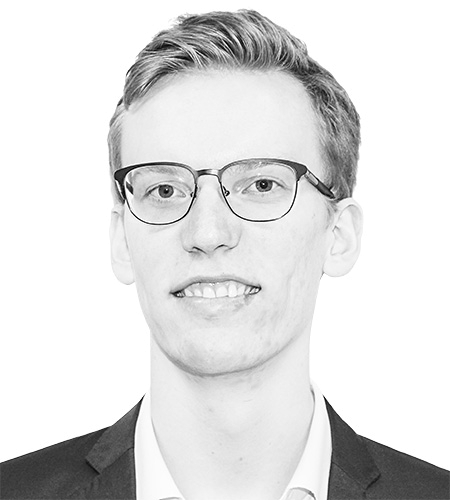
\includegraphics[scale=0.38]{profile}}}
	\end{picture}

	\begin{tabular}{Dl}
		\textsc{Address:}	&	 Vänortsvägen 5, Luleå, Sweden \\
		\textsc{Phone:}		&	 +46 73 763 87 77\\
		\textsc{email:}		&	 \href{mailto:Claes.Gustaf.Andersson@gmail.com}{Claes.Gustaf.Andersson@gmail.com}\\
		\textsc{LinkedIn:}	&	 \href{https://linkedin.com/in/ClaesGustaf}{linkedin.com/in/ClaesGustaf} \\
		\textsc{GitHub:}		&	 \href{https://github.com/Fizzr}{GitHub.com/Fizzr}
	\end{tabular}

	%\section{Goal}
	%{\small The main goal in my career is to learn. I want to be challenged in a way that forces me to learn new things and think in new ways. I want to become the best in my field at what I do, and I want to be a part of creating flawless and perfect solutions!}

	%Section: Education
	\section{Education}
	\begin{tabular}{D L{\textwidth-2.7cm}}
		\textsc{Jan 2020}	&	\textbf{Computer Engineering Master's Degree}\\
		\textsc{Aug 2012}	&	 \emph{Information and Communication Technology}. Luleå Tekniska Universitet.\\
		&	{\small Focus on Algorithms, Design paradigms, high levels of abstraction, Networking, and Internet services and development.}\\

		\textsc{Aug 2019} & \textbf{Master's Thesis}, \href{http://www.diva-portal.org/smash/record.jsf?pid=diva2%3A1350545}{Link}\\
		&                \emph{Predictive Model for Traffic Control in Underground Mines}, Luleå University of Technology, Mobilaris MCE\\
	\end{tabular}


	%Section: Work Experience
	\section{Work Experience}
	\begin{tabular}{D L {\textwidth - 2.7cm}}

		\textsc{Dec 2019}	&	\textbf{Software Developer}		\\
		\textsc{Jun 2017}	&	Mobilaris Mining and Civil Engineering	\\
		&	{\small Started as a summer job developing a POC for a cross-platform mobile version of the existing underground positioning system. Running on native C++ on an Android tablet and using OpenGL the POC ran smoother and was more responsive than the existing desktop version. After the summer job and POC was completed the project was assigned a team of seven people, made into a product and considered the company's highest priority. I was kept on working part time while completing my studies. Did my Master Thesis at Mobilaris, in which mine traffic is predicted by processing millions of logs. Mainly using C++ and CMake, some Python, and LaTeX. After completion I worked on a new POC of displaying a heatmap of data in the mine map using Unity, which also quickly became an important product.}\\
		\\

		\textsc{Oct 2018}	&	\textbf{Co-founder}		\\
		\textsc{Sep 2013}	&	DC Technological Innovations HB	\\
		&	{\small A company created in an attempt to bring Bitcoin to our university and make it the dominant payment method within campus.}\\
		\\

		\textsc{Jun 2017} 	& 	\textbf{Brand Ambassador} \\
		\textsc{Mar 2015}	&	Academic Work \\
		&	{\small Participating in different events and career fairs to recruit candidates. The job requires good communication skills and teamwork.}\\
		\\

		\textsc{Aug 2016}	&	\textbf{Junior Developer}\\
		\textsc{Jun 2016}	&	isMobile\\
		&	{\small Summer job. Worked with developing a demo suite for their Android Application Module. Primarily used XSLT, HTML, JavaScript, Java and LaTeX}	\\


	\end{tabular}

	%Section: Languages
	\section{Languages}
	\begin{tabular}{R{2cm} C{2cm} C{2cm}}
		\textsc{Fluent:}	& Swedish	& English\\
	\end{tabular}

	\section{Computer Skills}
	\def\arraystretch{1.2}%  Vertical space between tabs. 1 is the default
	\begin{tabu}{R{2cm} X[c] X[c] X[c] X[c] X[c]}
		\textsc{Languages:}		&	C++		& C\#		&   JavaScript	&	Python	&   Go 	\\
								&	Bash	&   Haskell	&	Java 	&	Prolog \\
		\textsc{Other:}			&	LaTeX	&   Git		&	OpenGL		& 	Unity	&	Linux\\
				        		&	CMake	&	Android	&	Blender &	3ds Max		\\
	\end{tabu}
	\vspace{0.1cm}

	\centering\textsc{ References available upon request}

\end{document}
